\documentclass[a4paper,12pt]{report}
%general packages
\usepackage[T2A]{fontenc}
\usepackage[utf8]{inputenc}
\usepackage[english,russian]{babel}
\usepackage{circuitikz}
\usepackage{wrapfig}
\usepackage{makecell}
\usepackage{tabularx}
\usepackage{graphicx}
\usepackage{gensymb}
\usepackage{cancel} %cancel symbol
\usepackage{amsmath,amsfonts,amssymb,amsthm,mathtools}
\usepackage[dvipsnames]{xcolor}


%\usepackage{epstopdf} %converting to PDF
%\usepackage{auto-pst-pdf}

%fancy header + geometry
\usepackage{fancyhdr}
\usepackage[a4paper,includehead,nomarginpar,left=15mm,right=15mm,top=15mm,headheight=10mm,bottom=20mm]{geometry}

%pgfplots
\usepackage{pgfplots}
\usepackage{pgfkeys}
\pgfplotsset{compat=1.12}
\usepackage{mathrsfs}

%multi column text
\usepackage{blindtext}
\usepackage{multicol}

%tikz (draw)
\usepackage{tikz}
\usepackage{pstricks-add}
\usetikzlibrary{intersections}
\usetikzlibrary{arrows.meta}
\usetikzlibrary{calc,angles,positioning}
\usetikzlibrary{arrows}
\usepackage{float}
\usepackage{filecontents}

%parskip settings
\parindent=0ex
\setlength{\parskip}{\baselineskip}%
\setlength{\parindent}{0pt}%

%fancy notation for sets
\newcommand{\R}{{\mathbb R}}
\newcommand{\N}{{\mathbb N}}
\newcommand{\fancy}[1]{{\mathbb{#1}}}
%sgn function
\DeclareMathOperator{\sgn}{sgn}

% intersection and union symbols
\newcommand{\uni}{\cup}
\newcommand{\inter}{\cap}
\newcommand{\re}{\text{Re}}
\newcommand{\const}{\text{const}}

\renewcommand{\footrulewidth}{0.4pt}

%\newcommand{\celsius}{$\ ^\circ C$}

%environments

\newtheorem{problem}{Задача}[]
\newenvironment{sol}{\paragraph{Решение}}{}
\renewcommand\thesection{\arabic{section}}

\usepackage{titlesec}
\titlespacing*{\section}
{0cm}{\baselineskip}{0pt}
\titlespacing*{\subsection}
{0pt}{0.1\baselineskip}{0.1\baselineskip}
\titlespacing*{\paragraph}
{0pt}{0.1\baselineskip}{\baselineskip}

\setcounter{secnumdepth}{0}

\begin{document}
	

\begin{titlepage}
	\begin{center}
		МОСКОВСКИЙ ФИЗИКО-ТЕХНИЧЕСКИЙ ИНСТИТУТ (НАЦИОНАЛЬНЫЙ ИССЛЕДОВАТЕЛЬСКИЙ УНИВЕРСИТЕТ) \\
		
		
		\hfill \break
		Факультет обшей и прикладной физики\\
		\vspace{2.5cm}
		\large{\textbf{Отчёт по лабораторной работе 1.2.5 <<Исследование прецессии уравновешенного гороскопа>>}}\\
		\hfill \break
		\\
	\end{center}
	
	\begin{flushright}
		Выполнил:\\
		Студент гр. Б02-304\\
		Головинов. Г.А.
	\end{flushright}
	
	\vspace{7cm}
	
	\begin{center}
		
\includegraphics[width=0.15\linewidth]{uni}
	\end{center}
	

	

	\vfill
	
	\begin{center} Долгопрудный, 2023 \end{center}
	
	\thispagestyle{empty}
	
\end{titlepage}


	\newpage
	%\pagenumbering{arabic}
    \pagestyle{fancy}

    \fancyhead{}
    \fancyfoot{}
    \fancyhead[L]{\rightmark}
    \fancyhead[R]{\thepage}
    \fancyfoot[R]{Работа 2.4.1. --- определение теплоты испарения жидкости}

    \section*{Аннотация}
        \paragraph*{Цель работы:} 1) измерить давление насыщенного пара жидкости при разной температуре; 2) вычислить по полученным данным теплоты испарения с помощью уравнения Клапейрона---Клаузиуса.
        \paragraph*{В работе используются:} термостат, герметичный сосуд, исследуемая жидкости, отсчетный микроскоп. 
    \vspace{0.5cm}
    \hrule

    \section{Основные теоретические сведения}


    \begin{multicols}{2}

    Получим условие равновесия двух фаз:

    Пусть $N_1, N_2$ --- количество частиц в фазах 1 и 2, а $V_1, V_2$ --- объемы, тогда
    \begin{equation}
        \label{dN}
        dN_1=-dN_2, \quad dV_1=-dV_2
    \end{equation}
    Запишем для обеих фаз изменение внутренней энергии:
    \begin{gather*}
        dU_1=TdS_1-pdV_1+\mu_1 dN_1 \\
        dU_2=TdS_2-pdV_2+\mu_1 dN_2
    \end{gather*}
    сложим предыдущие равенства и получим слева ноль в силу изолированности системы.
    \begin{equation*}
        T(dS_1+dS_2)-p(dV_1+dV_2)+\mu_1 dN_1 + \mu_2 dV_2 = 0
    \end{equation*}
    в силу \eqref{dN} получим
    \begin{equation*}
        T(dS_1+dS_2)=(\mu_1-\mu_2)dV_2
    \end{equation*}
    в равновесии энтропия максимальна, значит $dS_1+dS_2=0$, отсюда получим условие равновесия двух фаз:
    \begin{equation}
        \label{condition}
        \mu_1(p,T)=\mu_2(p_T)
    \end{equation}
    Теперь можно расписать изменение химических потенциалов:
    \begin{gather*}
        d\mu_1=-s_1dT+v_1dp
        d\mu_2=-s_2dT+v_2dp
    \end{gather*}
    Вследствие равенства самих потенциалов равны и их изменения:
    \begin{equation*}
        (s_2-s_1)dT=(v_2-v_1)dp
    \end{equation*}
    Отсюда получается соотношение Клапейрона---Клаузиуса:
    \begin{equation}
        \frac{dp}{dT}=\frac{s_2-s_1}{v_2-v_1}\cdot\frac{T}{T}=\frac{q}{T(v_2-v_1)}
    \end{equation}
    где $q$ --- удельная теплота фазового перехода при переходе из состояния 1 в состояние 2 (при испарении положительна, при конденсации отрицательна), $v_1, v_2$ --- удельные объемы в соответствующих состояниях.

    Для нашей работы актуальна следующая версия этого соотношения:
    \begin{equation}
        \label{clausius}
        \frac{dp}{dT}=\frac{L}{T(V_2-V_1)}
    \end{equation}
    где $p$ --- давление насыщенного пара при температуре $T$ --- абсолютная температура жидкости и пара, $L$ --- теплота испарения жидкости, $V_2$ --- объем пара, $V_1$ --- объем жидкости. Все величины относятся к одному молю вещества.

    Объем жидкости $V_1$ намного меньше чем объем пара $V_2$ (менее 0.5\% от $V_2$). Поэтому $V_1$ можно пренебречь.

    Объем $V_2$ теперь будем просто обозначать $V$. Его можно связать с давлением и температурой уравнением Ван-дер-Ваальса:
    \begin{equation}
        \label{vdv}
        \left(p+\frac{a}{V^2}\right)(V-b)=RT
    \end{equation}
    табличная величина $b$ тоже достаточно мала (соизмерима с $V_1$, которым мы пренебрегли), поэтому и ее мы учитывать не будем.
    
    Пренебрежение $a/V^2$ дает ошибку менее 3\%, при давлении ниже атмосферного ошибка становится еще меньше. Таким образом, будем считать насыщенный пар идеальным газом:
    \begin{equation}
        \label{ideal}
        pV=RT
    \end{equation}
    Подставляя \eqref{ideal} в \eqref{clausius} получим:
    \begin{equation}
        \label{L}
        L=\frac{RT^2}{p}\cdot\frac{dp}{dT}=-R\frac{d(\ln p)}{d(1/T)}
    \end{equation}
    \end{multicols}

    \hrule

    \section{Экспериментальная установка}
    \begin{figure}[H]
        \centering
        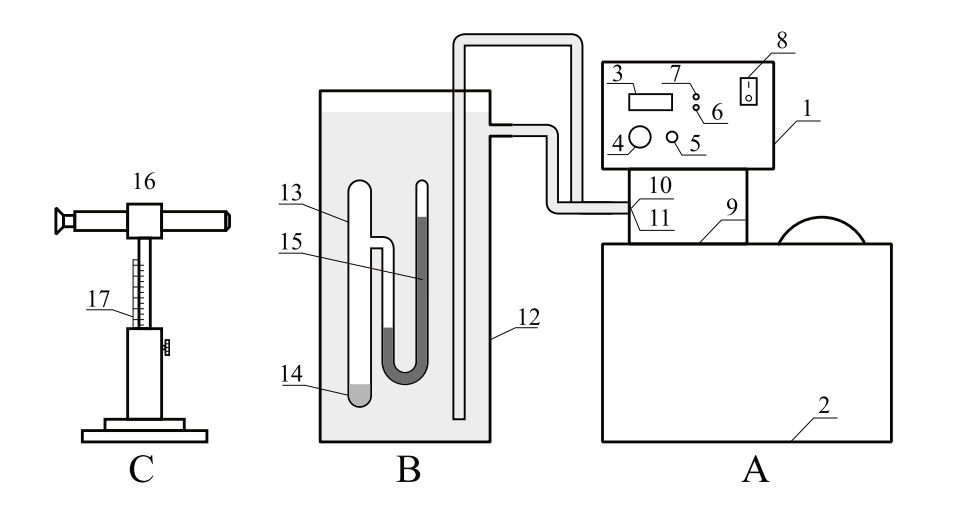
\includegraphics[width=0.9\columnwidth]{../img/experiment.png}
        \caption{Схема установки для определения теплоты испарения}
    \end{figure}
    Температура выставляется с помощью термостата А, давление измеряется при помощи экспериментального прибора B и микроскопа C: оно определяется с помощью ртутного манометра 15. Высоту столба (разницы столбов) мы измеряем с помощью микроскопа 16 и шкалы 17. 

\end{document}
